\subsubsection{Compara\c c\~ao dos modelos}

Com o objetivo de obter uma análise mais aprofundada do desempenho de cada modelo, foi realizada uma comparação por meio de um gráfico de violino. Dessa forma, pôde-se observar qual dos modelos apresentava o melhor desempenho.


\begin{figure}[!htpb]
	\centering
	\caption{Análise comparativa dos modelos utilizando gráficos de violino}
	\begin{subfigure}{0.9\textwidth}
		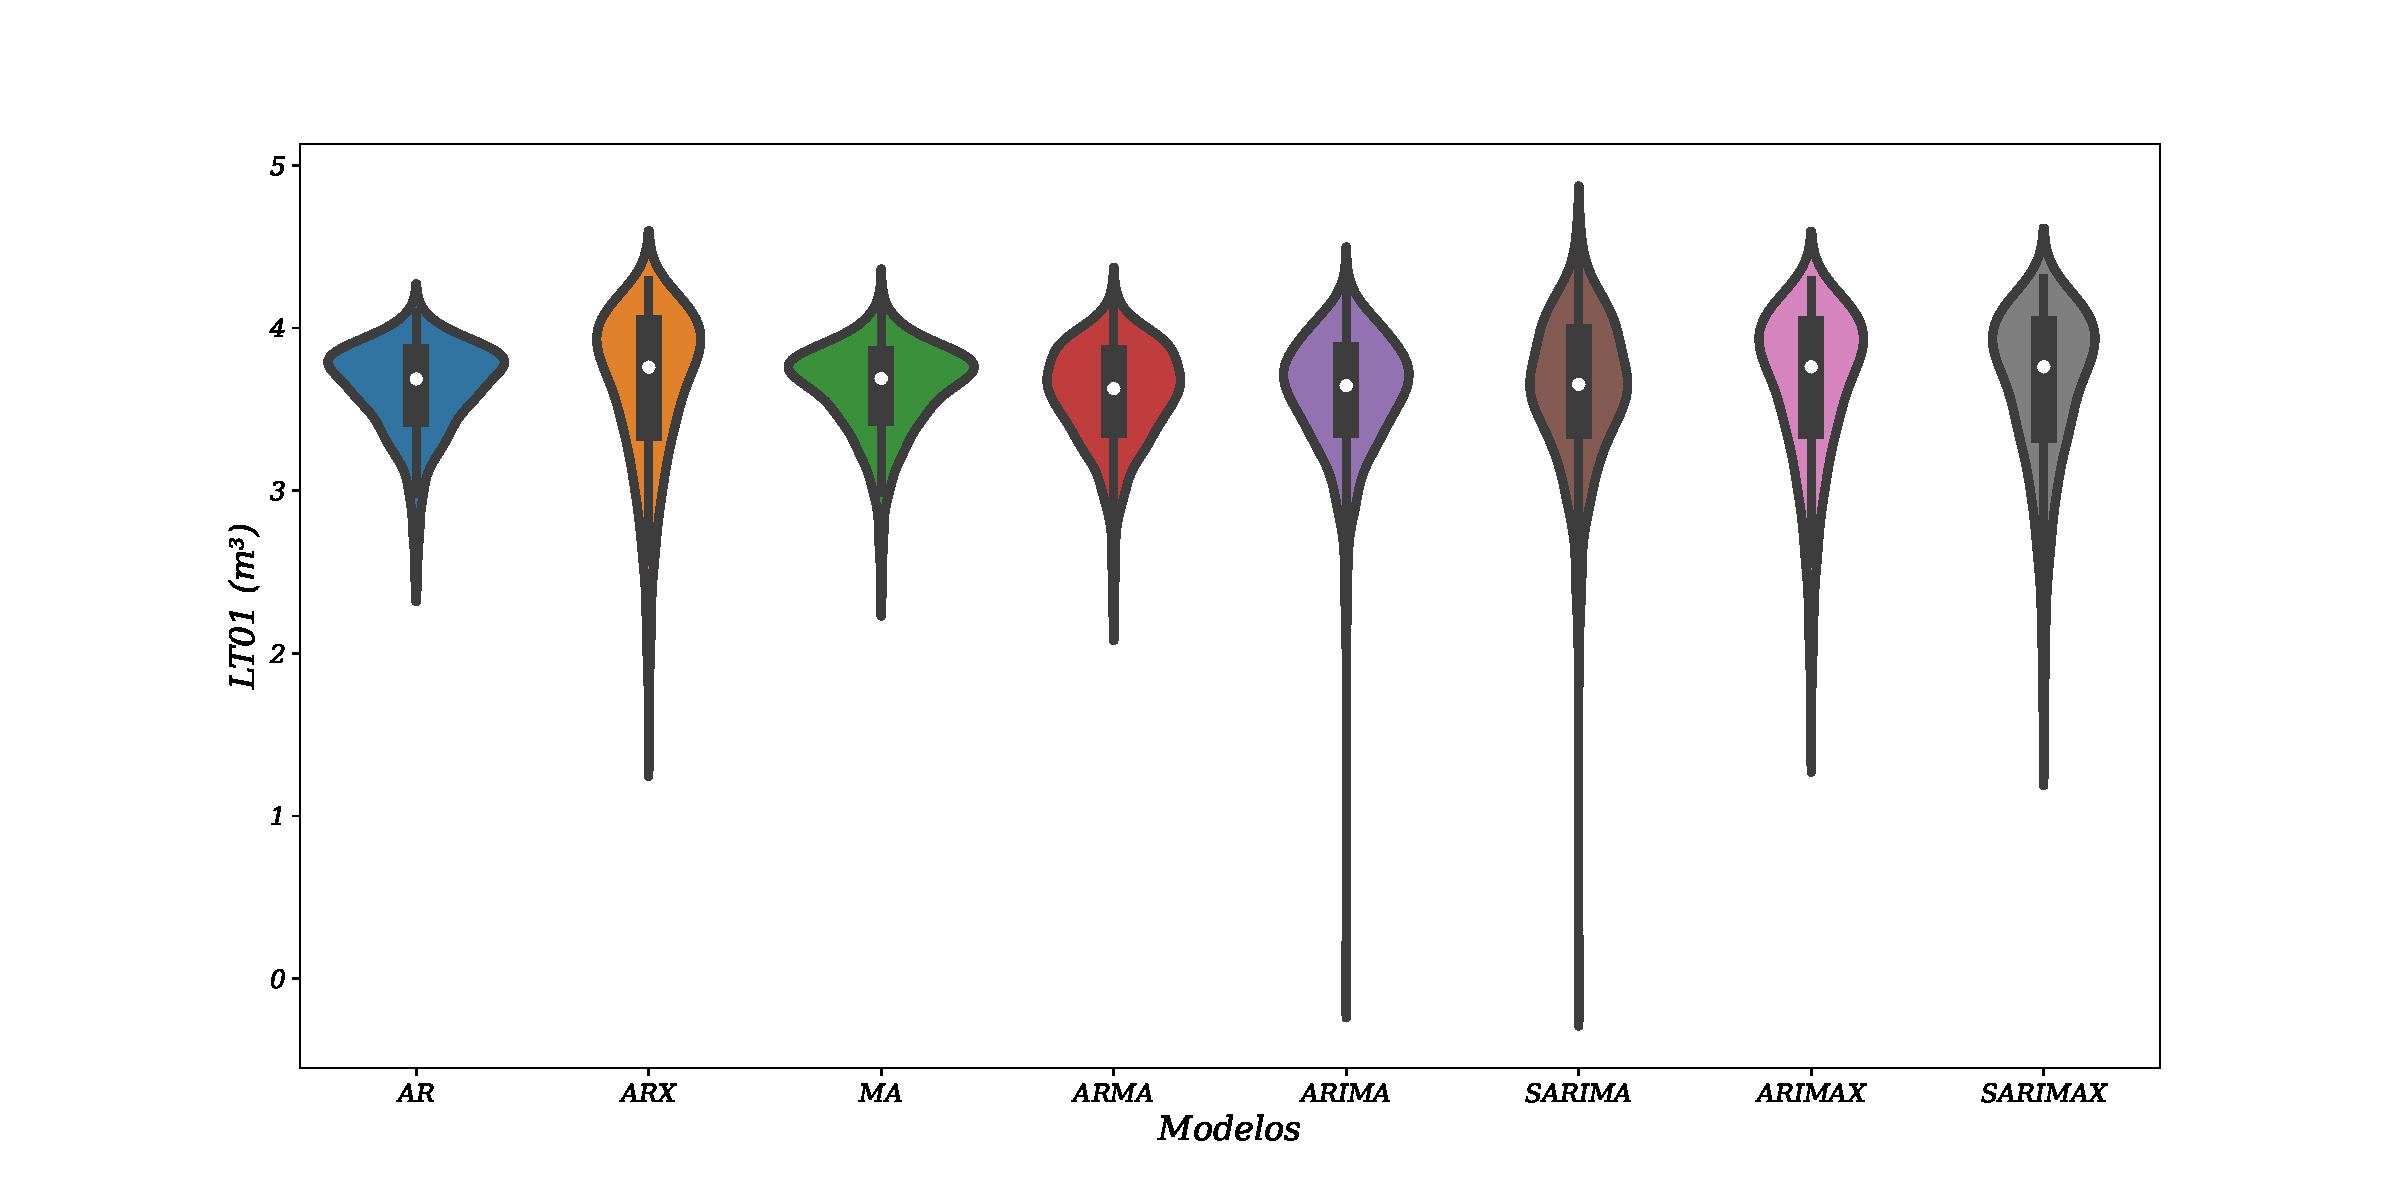
\includegraphics[width=\linewidth]{Resultados/Figuras/modelos-arima}
		\caption{Comparação dos modelos ARIMA}
		\label{fig:modelos-arima}
	\end{subfigure}
	
	\begin{subfigure}{0.9\textwidth}
		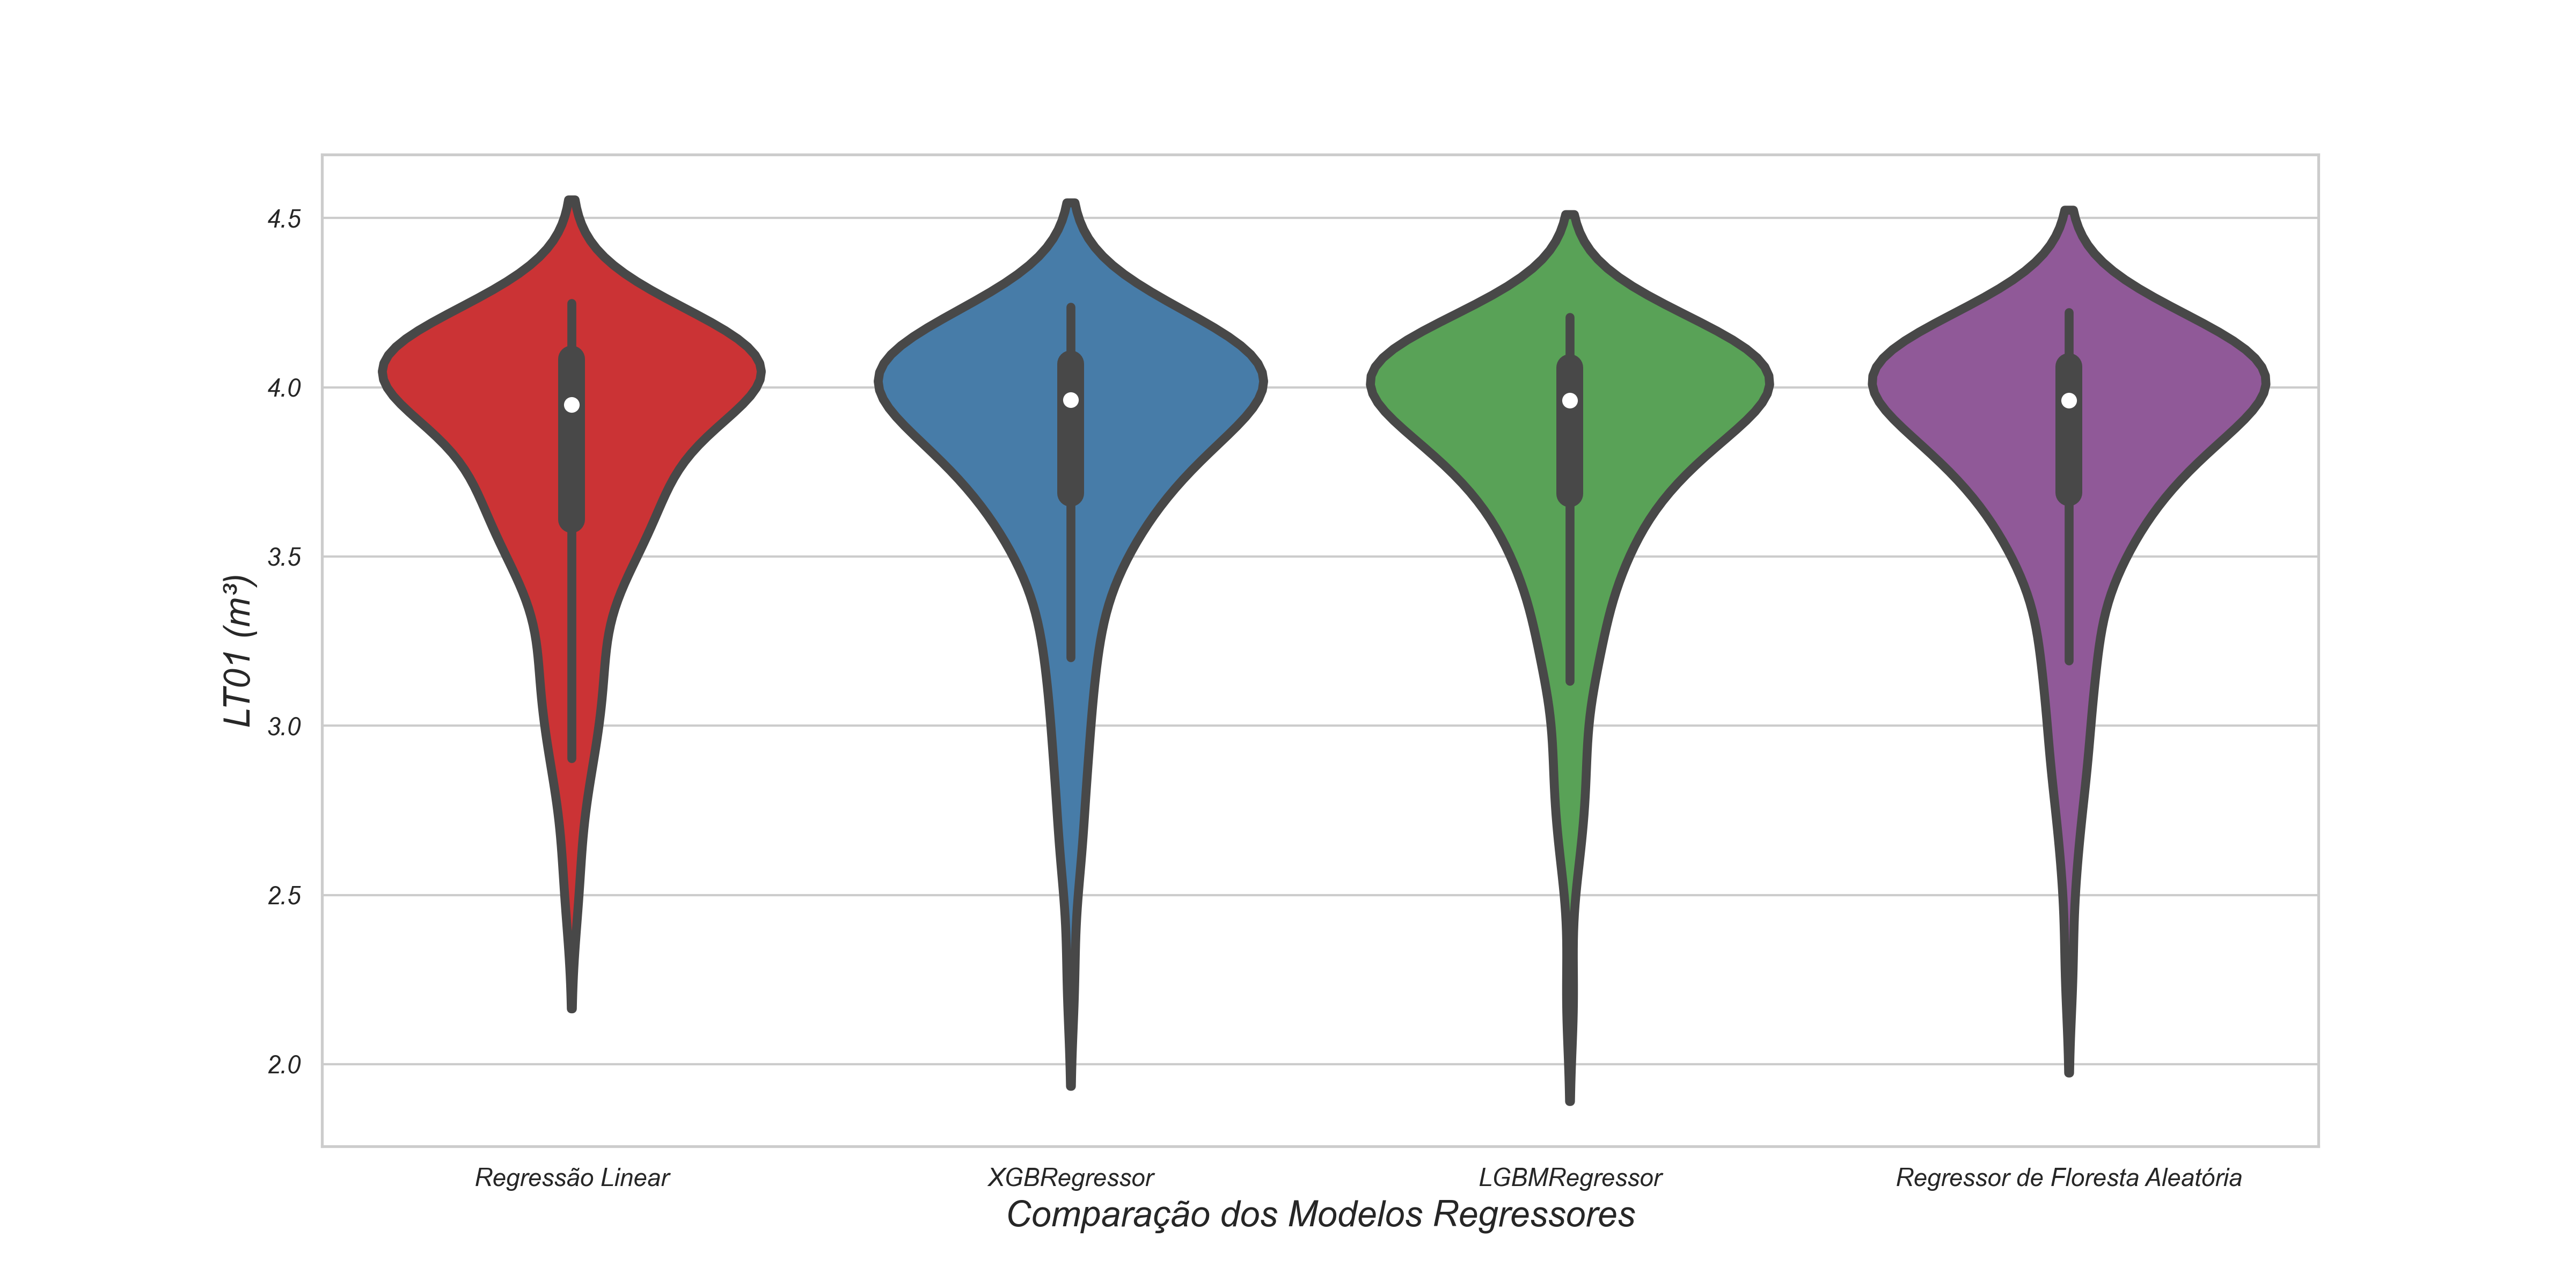
\includegraphics[width=\linewidth]{Resultados/Figuras/violin-LR-XGB-LGBM-RF}
		\caption{Comparação de modelos de regressão}
		\label{fig:violin-lr-xgb-lgbm-rf}
	\end{subfigure}
	
	\fonte{Elaboração própria a partir de dados da SANEPAR (2018 a 2020)}
\end{figure}

Ao comparar os modelos apresentados nas Figuras \ref{fig:modelos-arima} e \ref{fig:violin-lr-xgb-lgbm-rf}, é possível observar quais são os modelos que se destacam, levando em consideração a modelagem dos dados. Os modelos ARIMA que mostram melhor desempenho são o AR, ARX, MA, ARMA, ARIMAX e SARIMAX, devido à sua capacidade de lidar com \textit{outliers} e limites inferiores em alguns modelos. No caso dos modelos baseados em gradientes e regressão, é perceptível que eles exibem resultados semelhantes, graças às técnicas de otimização matemática conhecidas como Grid Search e Randomized Search, que permitem aprimorar os métodos utilizados.

Quando se trata de um horizonte de previsão curto, o modelo de LR apresenta melhor desempenho em comparação com os demais. No entanto, em horizontes de previsão mais longos, os modelos XGBoost e Light GBM demonstram maior precisão. A Random Forest também é capaz de realizar previsões precisas, ficando ligeiramente atrás do XGBoost em previsões de longo prazo.

Para avaliar a eficiência dos modelos ARIMA em previsões de longo prazo, utiliza-se o método conhecido como Ljung-Box, como apresentado no apêndice \ref{sec:comtb18}. As Tabelas de \ref{tb:lbtrn} a \ref{tb:lbcm} mostram a precisão dos modelos ARIMA ao longo do tempo, destacando em \textbf{negrito} os números menores para facilitar a compreensão. Os modelos ARX, ARIMAX e SARIMAX, que incorporam variáveis exógenas, demonstram um melhor desempenho nesse contexto. Esses modelos não lineares possuem uma capacidade de previsão mais robusta em horizontes de tempo mais distantes, em comparação com os outros modelos ARIMA.
